\documentclass[11pt]{article}
\usepackage{amsmath}
\usepackage{amsfonts}
\usepackage{amssymb}
\usepackage[margin=1in, paperwidth=8.5in, paperheight=11in]{geometry}
\usepackage{fancyhdr}
\usepackage{graphicx}
\usepackage{mathtools}

\pagestyle{fancy}
\fancyfoot{}
\fancyhead[L]{\slshape Peter Wu}
\fancyhead[C]{\slshape pwu052@uottawa.ca}
\fancyhead[R]{\slshape 8916747}
\fancyfoot[R]{\thepage}

\begin{document}
\begin{center}
\begin{Large}
Assignment 4 Report
\end{Large}
\end{center}
For this assignment, I am asked to read a given file containing subway stations and lines, then traverse through the graph to identify the line starting from the station entered by user, compute the shortest path between two stations user entered, and the shortest path if one station malfunctions.\\
\\
I have used net.datastructures implemented by Goodrich et al. (specifically, AdjacencyMapGraph to store the graph, HeapPriorityQueue to store the distances for computing shortest paths, and ProbeHashMap to store all the vertices in the cloud) and some lab solutions to solve this assignment. I have also used an array list to store all vertices on the same line as the malfunction station.\\
\\
To identify the line, one should do the Depth-First traversal to the graph. The idea is to start from the source and visit the next vertex connected to the source vertex, and mark this vertex as visited and set this vertex as the new starting point. We keep doing this traversal until we have visited all vertices on the line. I used a hash table to store all visited vertices so that if we encounter a cycle we will exit the traversal.\\
\\
For computing the shortest path, one can use Dijkstra's algorithm. The algorithm simply calculates the shortest distances(time in this assignment) to every other vertices the source vertex can reach. We have a cloud of visited vertices(vertices that already have the shortest distance computed). Initially our cloud has only one vertex, which is the source vertex, it has a distance 0 since traveling from the source vertex to the source vertex has a distance 0 and it is indeed the shortest distance. Then we set distances to all other vertices to $\infty$ since we have not visited them yet and we have not calculated the distances. Once we start visiting vertices, we will perform edge relaxation step, where we update the shortest distance by comparing the original shortest distance with the new distance with the weight of edges added to it. If the new distance is shorter, then the new shortest distance will be that distance, and the new vertices will be added to the cloud. In the case where a station malfunctions, we simply skip the vertices that are on the same line as our malfunction station while performing edge relaxation so that these vertices will not be in the cloud. \\
\\
To show the shortest path from one vertex to another, I have used an array storing integers(since our vertices are represented as integers). Each index represents the vertex, and the content of each index is the previous vertex along in the shortest path. Whenever an edge relaxation step happens, I will add the previous vertex(current source vertex) to this array at the vertex index(current destination vertex). Then I print it by reversely tracing the indexes starting with the destination vertex.\\
\\
Here are some examples of the outputs of my program:\\
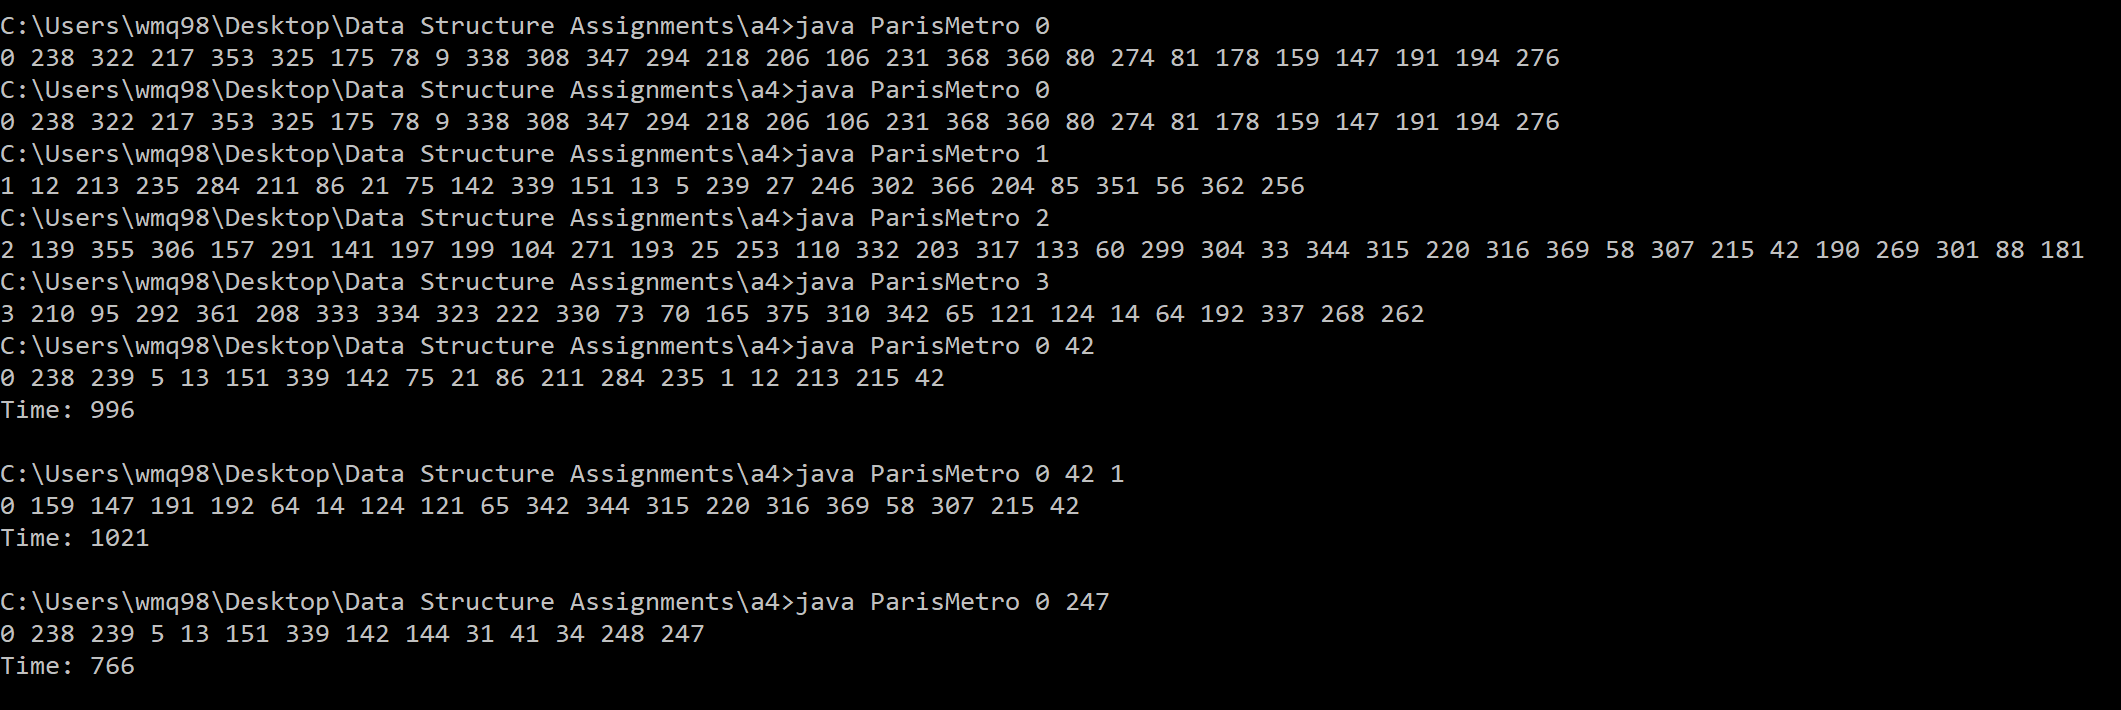
\includegraphics[scale=.5]{Screenshot1.png}\\
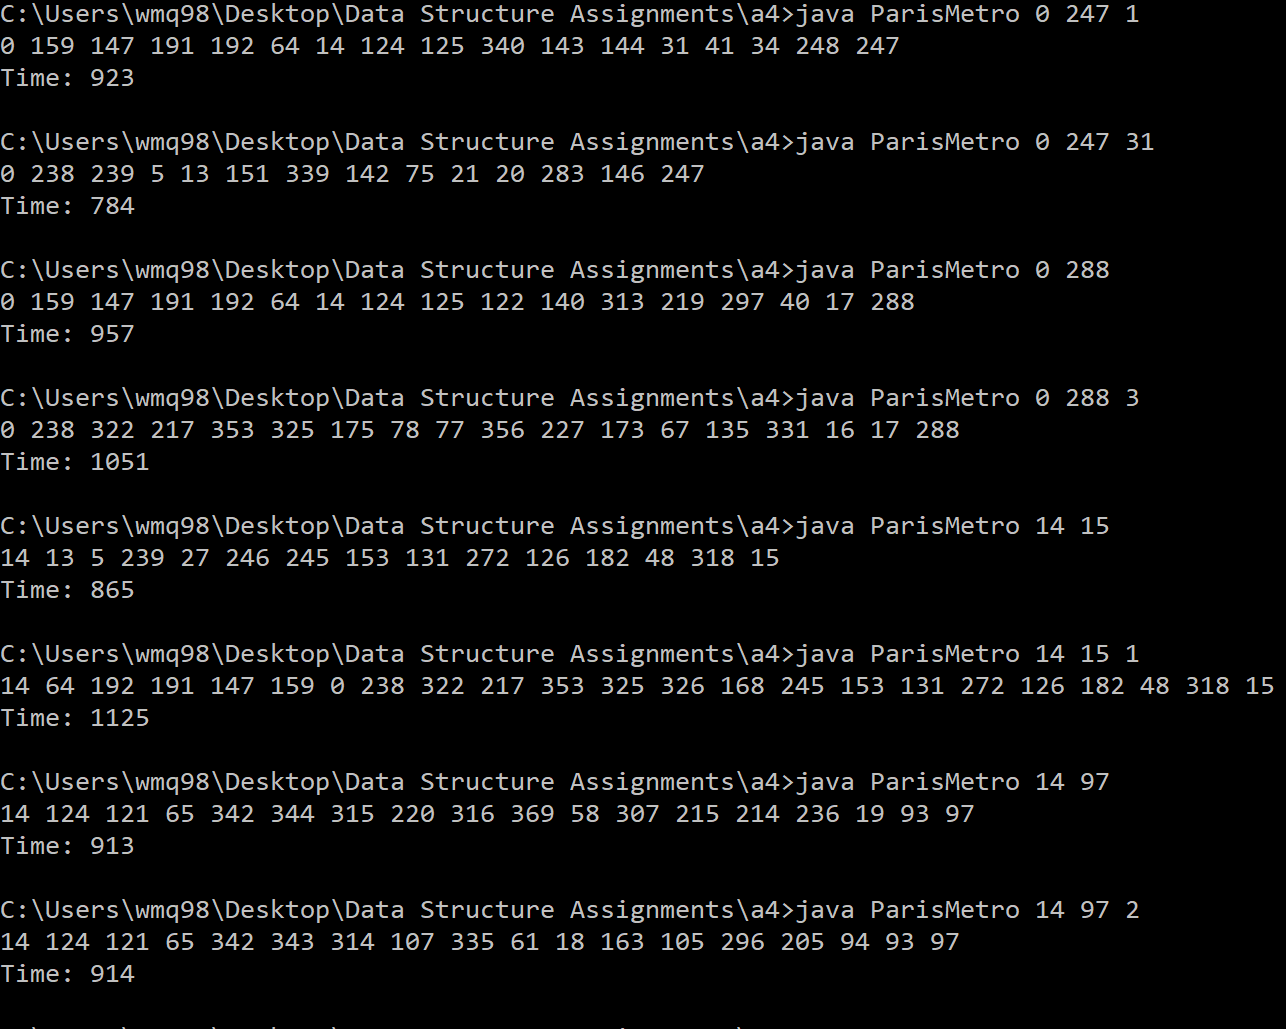
\includegraphics[scale=.5]{Screenshot2.png}\\
(References concerning the methods I used from other sources are available in the comments of my program).

\end{document}